\setcounter{section}{0}
\renewcommand{\thesection}{\Alph{section}}

% \maketitle

\section*{\Large Appendix}
This appendix provides experimental details, results, and analyses that complement the main paper. 
\begin{itemize}
\item Section~\ref{sec:appendix-experimental_settings} describes the training data, implementation details, simulation and real-world evaluation settings, baseline settings, and inference benchmark protocol.
\item Section~\ref{sec:appendix-additional_results} presents additional simulation benchmark results on LIBERO, LIBERO-Plus, and RoboCasa.
\item Section~\ref{sec:appendix-ablation_analysis} provides additional ablations and analyses, including backbone variants, pre-training ablations, split-layer analysis, action-token attention, and robustness trends.
\end{itemize}

\label{secA}

\section{Experimental Settings and Reproducibility Details}
\label{sec:appendix-experimental_settings}

GAM is trained in two stages, following standard practice for generalist robot policies~\citep{openvla_oft, black2024pi_0}. The first stage jointly trains the predictor, action head, and the GFM backbone end-to-end on a large mixture of single-arm robot data. The model was trained using 64 NVIDIA GH200 GPUs witch batch size of 1024, which takes approximately \textasciitilde 96 hours. The second stage fine-tunes the entire model on each benchmark's official training set before evaluation. The second stage on simulation benchmark was trained using 16 NVIDIA GH200 GPUs with batch size of 160, which takes \textasciitilde 48 hours.
\subsection{Pre-training Details}
\label{sec:appendix-pretraining_details}
We pre-train GAM on a weighted mixture of Open-X Embodiment~\cite{collaboration2023open} (OXE), MimicGen~\cite{mandlekar2023mimicgen}, and RoboCasa365~\cite{nasiriany2026robocasa365}. OXE provides broad real-robot coverage across multiple embodiments and manipulation domains, while MimicGen and RoboCasa365 provide simulation demonstrations with clean geometric supervision. The sampling ratios are 72\%, 18\%, and 10\% for OXE, MimicGen, and RoboCasa365, respectively. For future-depth supervision, we use teacher pseudo-depth for OXE and re-rendered simulator depth for MimicGen and RoboCasa365. Figure~\ref{supfig:training_data} shows the dataset mixture used for pre-training.

For OXE, we use the subset whose actions can be mapped to our common control interface and exclude datasets that are incompatible with our action space.. For RoboCasa365, we use only the manipulation-task subset. Across all three sources, we keep the original task language provided by the datasets and do not synthesize additional instructions. The language encoder is kept frozen during pre-training.

All datasets are converted to a common observation and action format before training. Images are resized to \(224\times224\), and the model uses two RGB views when available: an external view and a wrist view. Following Cosmos-policy~\cite{kim2026cosmos} and $\pi_{0.5}$~\cite{pi05}, standard image augmentations such as random cropping, rotation, and color jitter are applied during training and disabled during evaluation.


\begin{figure*}[h]
    \centering
    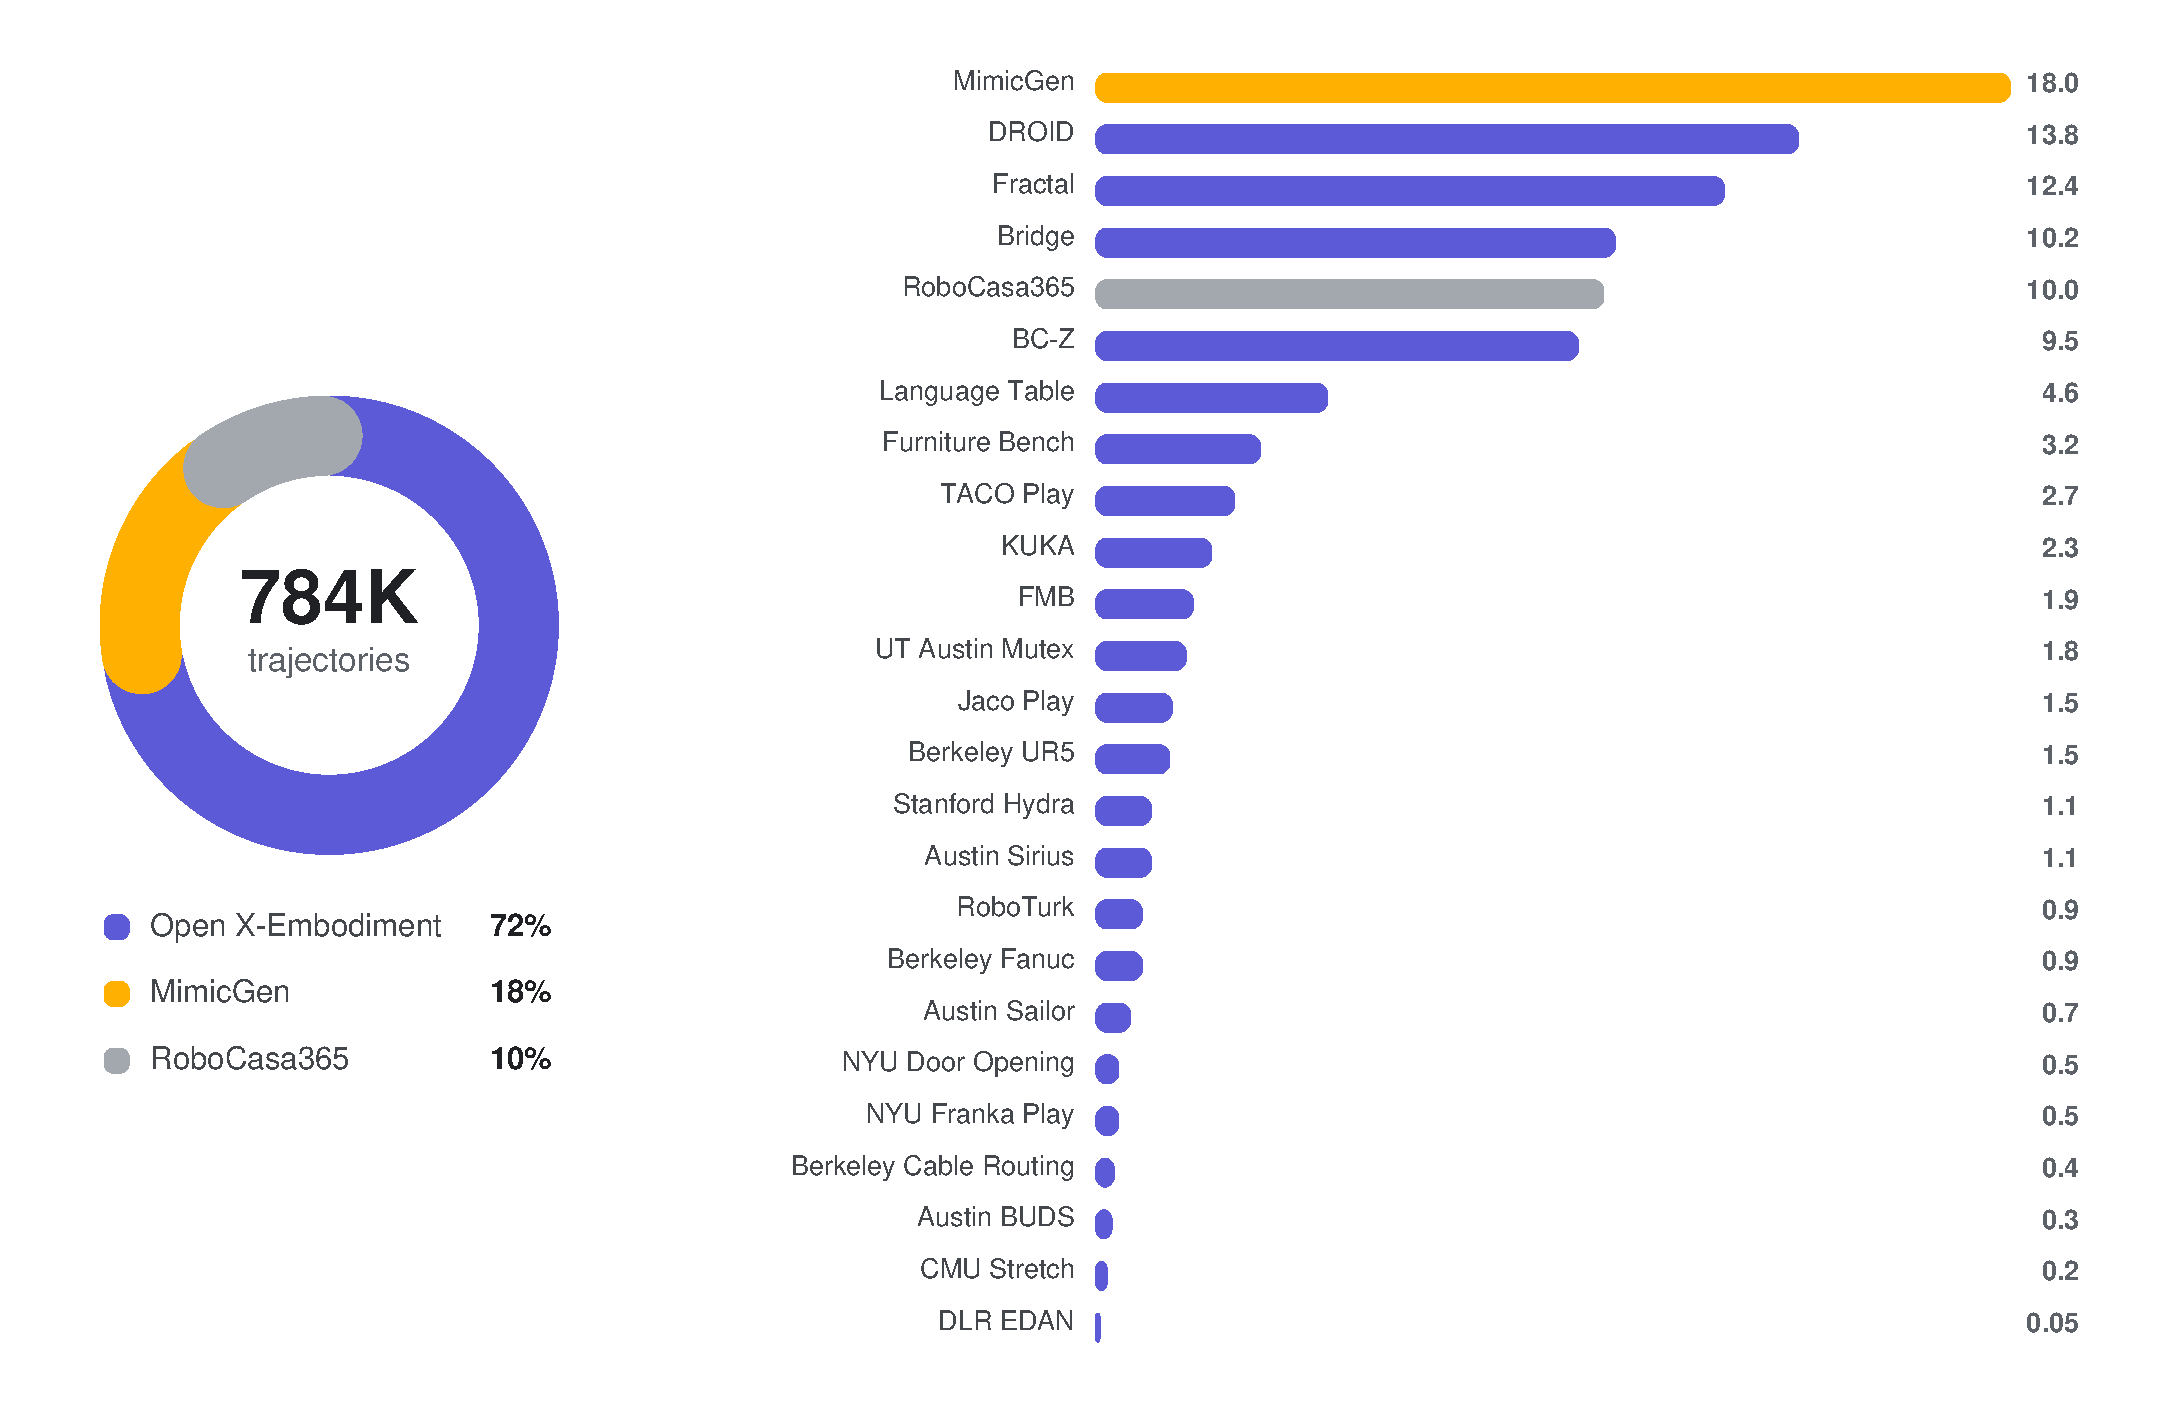
\includegraphics[width=\textwidth]{figures/data_ratio.pdf}
    \caption{
    \textbf{Training Dataset Mixture.} We illustrate the dataset mixture utilized during pretraining, detailing the relative proportions of each constituent dataset. The pie chart shows the high-level source mixture, and the bar chart shows the percentage of each constituent dataset relative to the entire training corpus.
    }
    \label{supfig:training_data}
\end{figure*}
\begin{table*}[t]
\centering
\caption{\textbf{Hyperparameters for LIBERO, LIBERO-Plus and real-world experiments.}}
\label{suptab:gam_hp}
\resizebox{1.0\linewidth}{!}{
\begin{tabular}{ll}
\toprule
hyperparameter & value \\
\midrule
\# GPUs & 8 $\times$ NVIDIA GH200 \\
learning rate (LR) & 5.16e-5 backbone; 5.16e-4 action head and predictor \\
total batch size & 160 \\
input images & 1 external camera image, 1 wrist-mounted camera image \\
input image size & 224 x 224 px \\
use observation history & no (use single-step inputs) \\
action chunk size & 8 steps (predict 8, execute all 8 open-loop at test time) \\
use proprio (robot state) & yes \\
\# trainable parameters & 983.2M total \\
image augmentations & 90\% random crop, $\pm5^\circ$ rotation, color jitter, JPEG q95: \\
& \;\; \texttt{random\_resized\_crop=dict(scale=[0.9, 0.9], ratio=[1.0, 1.0])} \\
& \;\; \texttt{base\_only\_rotation=[$\pm$5 deg]} \\
& \;\; \texttt{random\_brightness=[0.3]} \\
& \;\; \texttt{random\_contrast=[0.6, 1.4]} \\
& \;\; \texttt{random\_saturation=[0.5, 1.5]} \\
& \;\; \texttt{random\_hue=[0.05]} \\
& \;\; \texttt{jpeg\_quality=95} \\
\bottomrule
\end{tabular}}
\end{table*}


\subsection{Simulation Experiments Details}
\label{sec:appendix-simulation_details}
We adopt the LIBERO evaluation protocol established by OpenVLA~\cite{kim2024openvla} and OpenVLA-OFT~\cite{openvla_oft}. Specifically, we evaluate on the four standard LIBERO task suites: LIBERO-Spatial, LIBERO-Object, LIBERO-Goal, and LIBERO-Long, each consisting of 10 tasks. Following OpenVLA-OFT, we train on filtered LIBERO demonstrations by removing unsuccessful episodes and filtering idle/no-op frames, i.e., training samples with near-zero actions. We fine-tune a separate policy for each LIBERO suite. 

We report task execution success rate (SR, \%) as our primary evaluation metric. For the original LIBERO benchmark, each task is evaluated over 50 randomized trials, resulting in 500 rollouts per suite. For LIBERO-Plus, we follow the official evaluation setting and use one rollout per perturbed task instance. All models are trained with a global batch size of 160 for up to 110k training steps, until convergence is achieved. 
% Checkpoints are evaluated periodically throughout training, and we report the best-performing checkpoint for each run.

For baseline comparison, we re-evaluate $\pi_{0.5}$ and Cosmos-Policy under our evaluation setting using publicly available checkpoints. We also re-evaluate $\pi_{0.5}$ + Spatial Forcing and $\pi_{0.5}$ + ROCKET using reproduced checkpoints from ROCKET~\cite{sun2026rocket}. Results for the remaining baselines are taken from~\citet{fei2025libero} and ~\citet{zheng2026pokevla}.

\subsection{Real-World Experiments Details}
\label{sec:appendix-real_world_details}
Figure~\ref{supfig:real_world_setup} illustrates the experimental environment used for our real-world evaluations. Our hardware setup includes a wrist-mounted ZED Camera and an external RealSense camera providing a third-person perspective. 

\begin{figure*}[t]
    \centering
    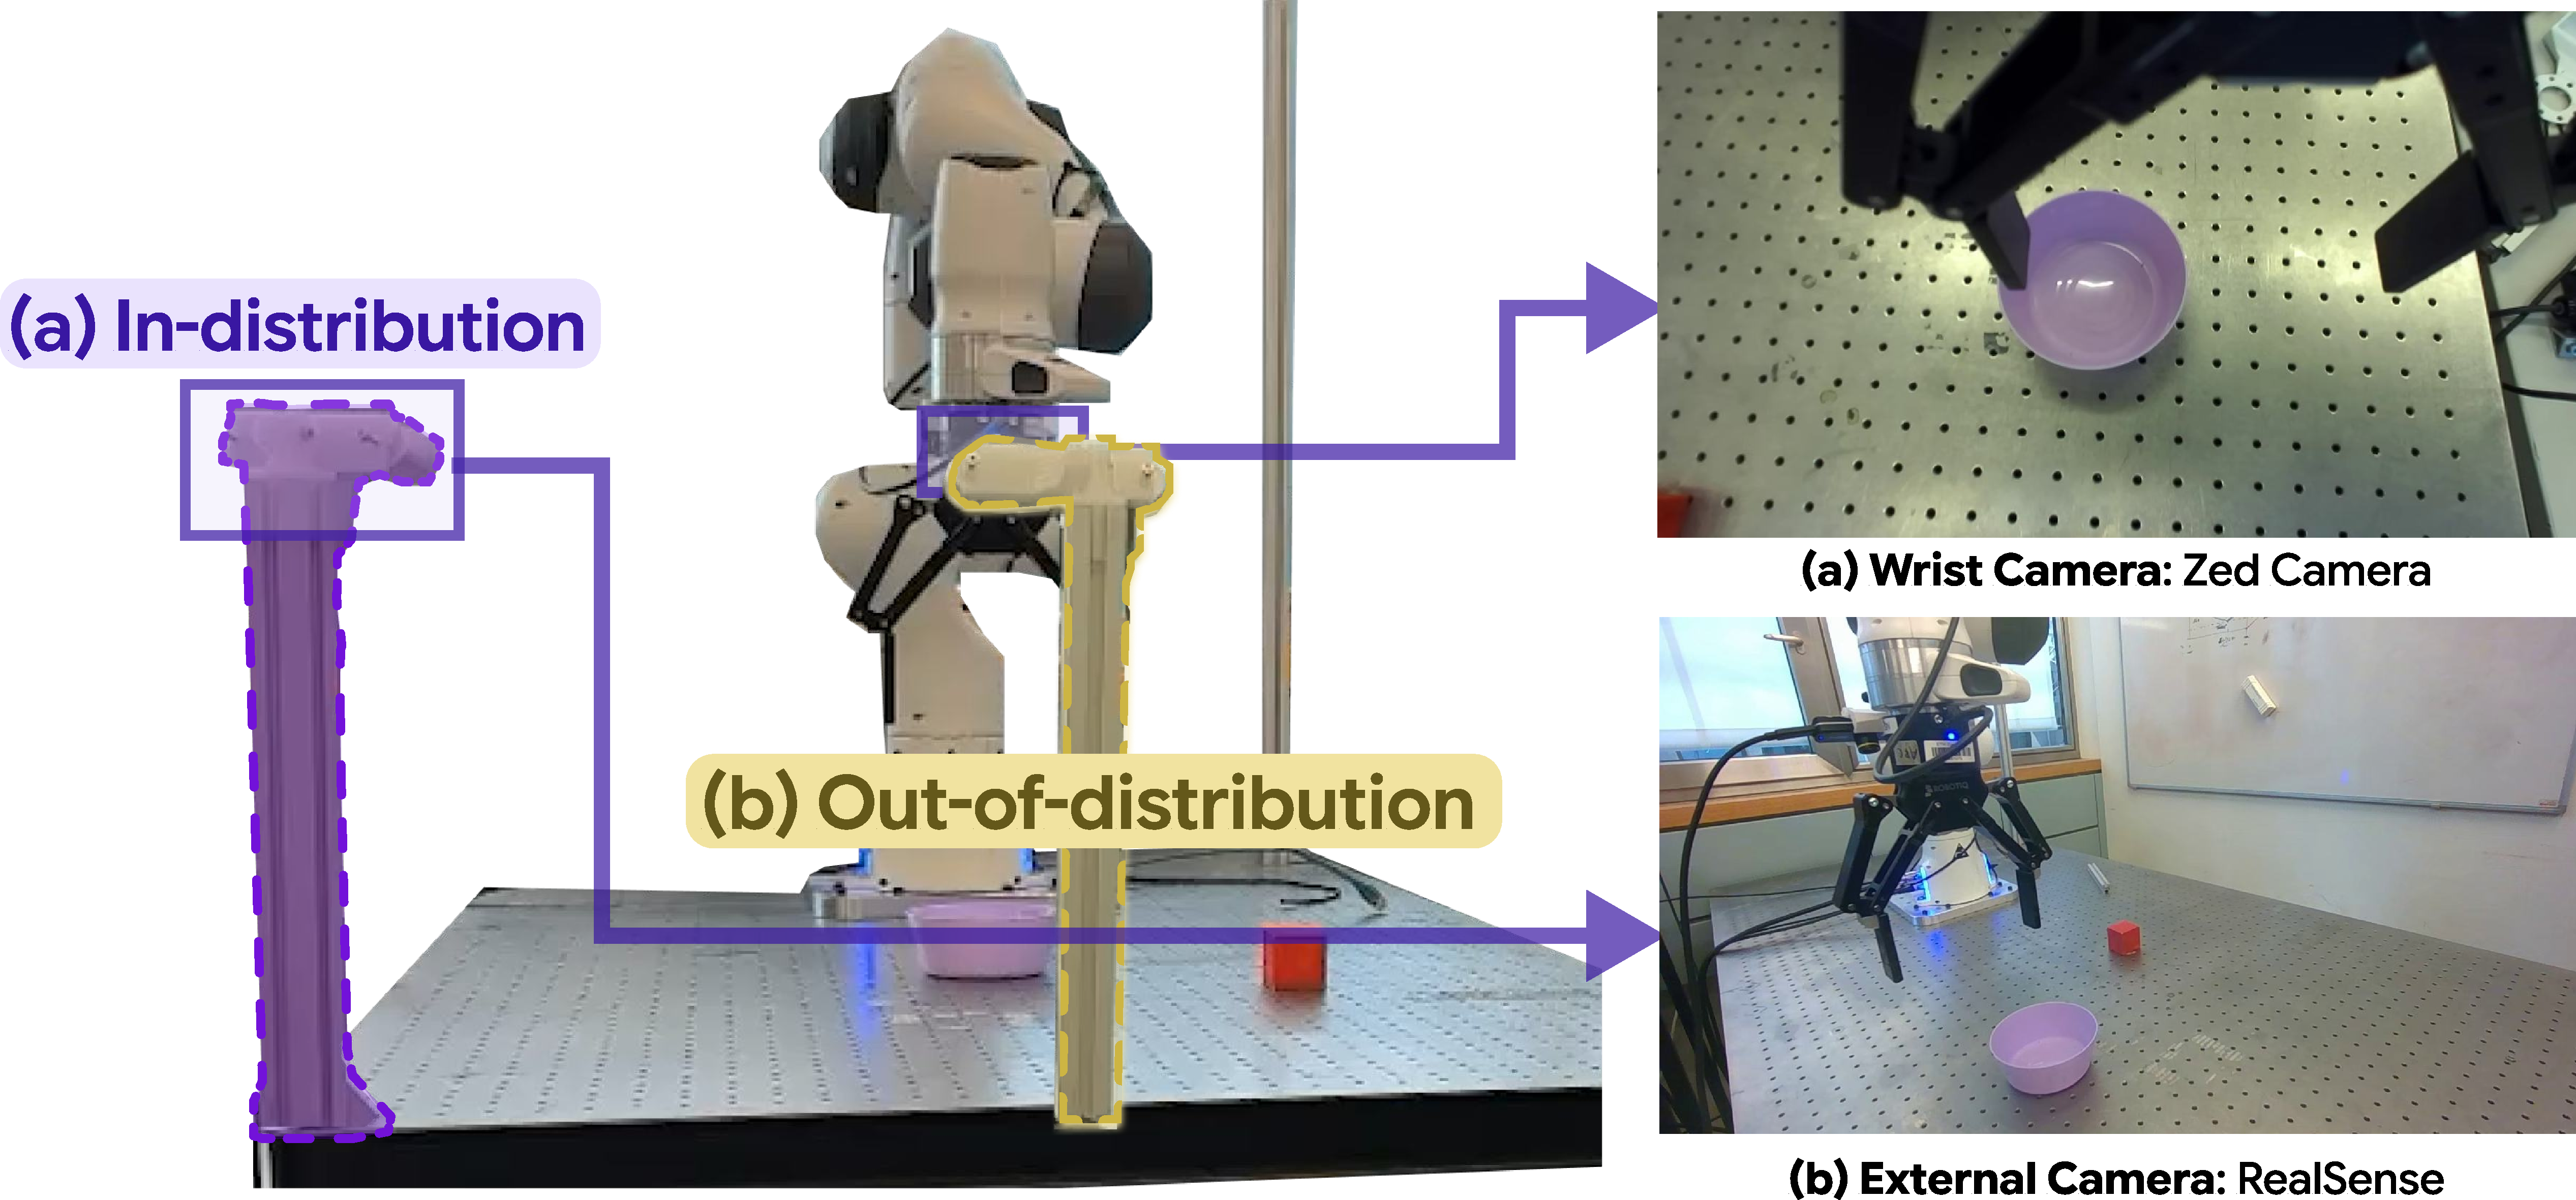
\includegraphics[width=\textwidth]{figures/physical_setup3.pdf}
    \caption{
    \textbf{Real-world experiments environment setup and ID vs. OOD Camera setup.}
    }
    \label{supfig:real_world_setup}
\end{figure*}


\begin{figure*}[t]
    \centering
    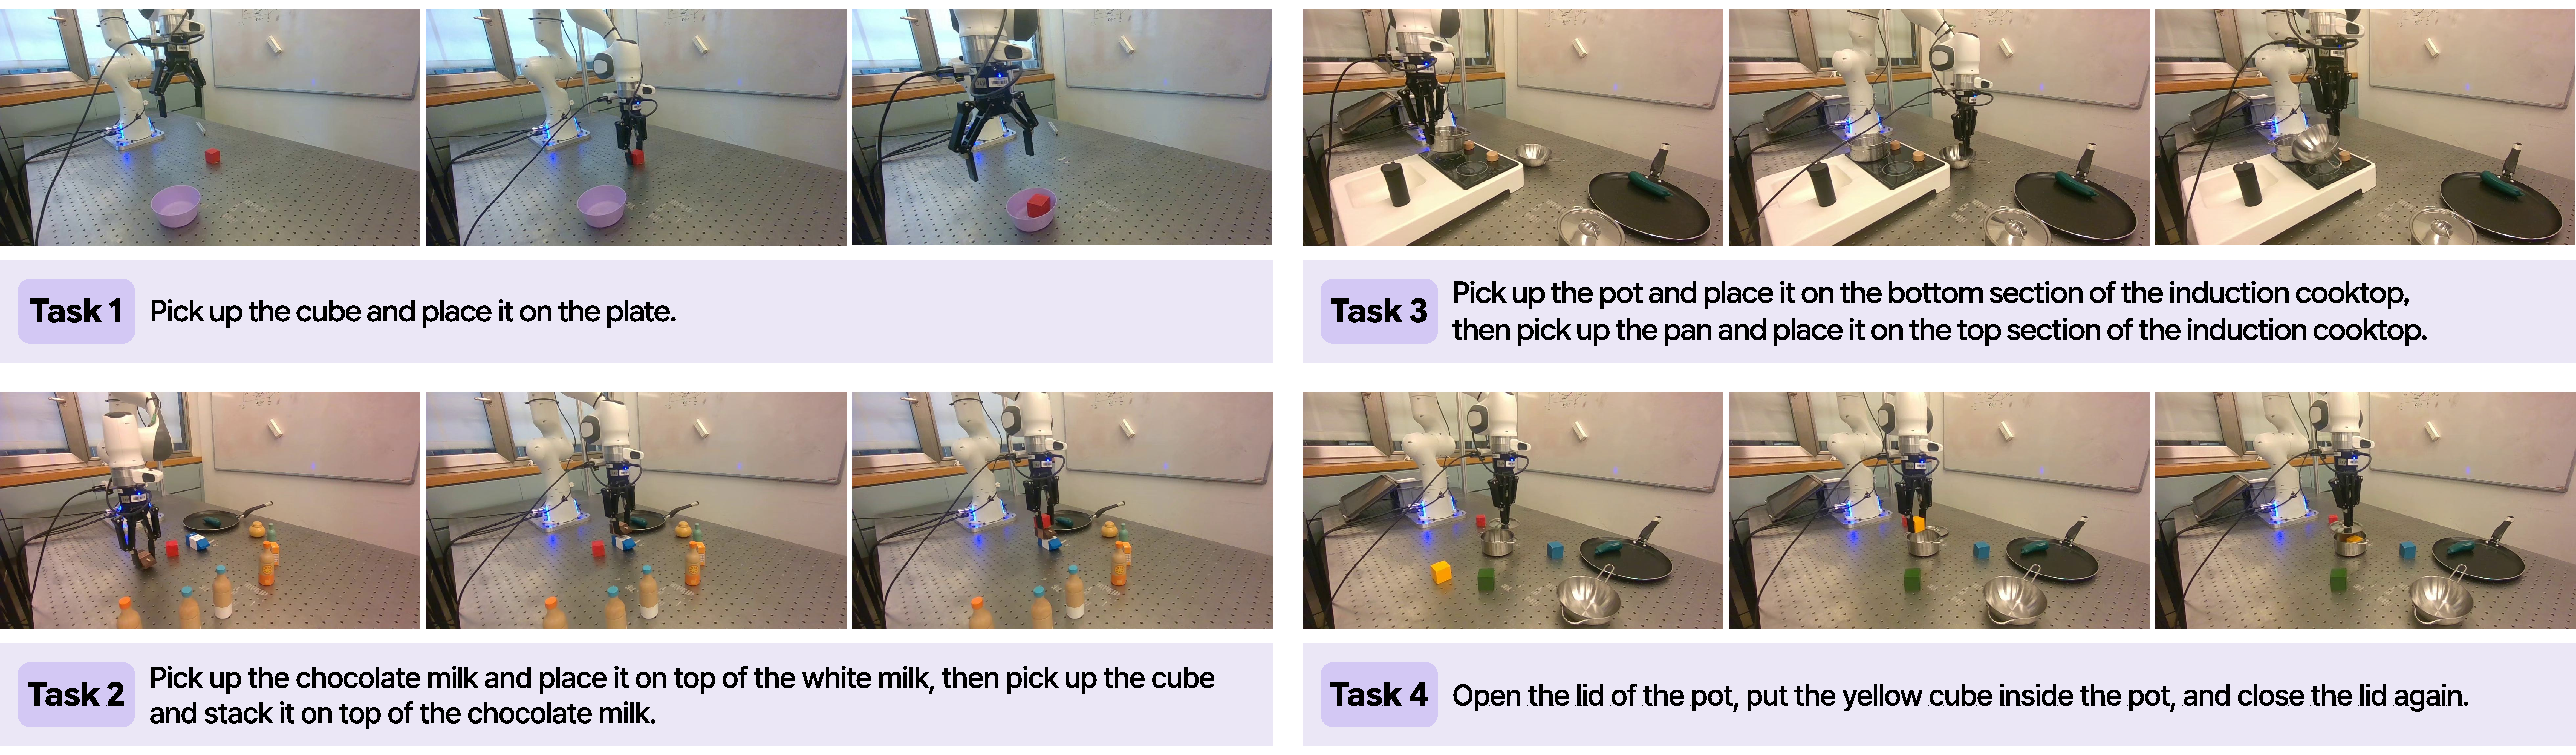
\includegraphics[width=\textwidth]{figures/tasks3.pdf}
    \caption{
    \textbf{Illustration of four real-world manipulation tasks.}
    }
    \label{supfig:real_world_tasks}
\end{figure*}

For training and evaluation, we defined four distinct tasks: Pick and place, Stack milk and cube, Place pot and pan on cooktop, and Insert cube into covered pot. We collected teleoperated demonstrations for each task: 284, 202, 184, and 169 demonstrations, respectively. Figure~\ref{supfig:real_world_tasks} shows the text instructions and corresponding visual illustrations for each task. All tasks were jointly trained within a unified dataset. The hardware specifications and hyperparameters used to train GAM, alongside the baselines ($\pi_{0.5}$~\cite{pi05} and Spatial Forcing~\cite{li2025spatial}), are detailed in Tables~\ref{suptab:gam_hp}, \ref{suptab:pi_hp}, and \ref{suptab:sf_hp}, respectively. All baseline models were trained until convergence using the default hyperparameters from the paper.


During evaluation, we measured the success rate of each task across 20 trials. Specifically, 10 trials were conducted under a normal setup (ID), while the remaining 10 trials evaluated robustness under an out-of-distribution (OOD) setup with camera perturbation. The camera perturbation was introduced by applying a translation of 85~cm and a rotation of 45$^\circ$ to the external camera shown in Figure~\ref{supfig:real_world_setup}. The left side of Figure~\ref{supfig:real_world_setup}, we provide a visualization comparing ID and OOD environment settings. This perturbation setup was kept consistent across all evaluations.


\begin{table*}[t]
\centering
\label{suptab:pi_sf_hp}
\scriptsize
\begin{minipage}[t]{0.49\linewidth}
\centering
\captionof{table}{\textbf{$\mathbf{\pi_{0.5}}$ hyperparameters.}}
\label{suptab:pi_hp}
\resizebox{\linewidth}{!}{
\begin{tabular}{ll}
\toprule
hyperparameter & value \\
\midrule
\# GPUs & 8 x NVIDIA H100 GPU \\
learning rate (LR) & 5e-5 \\
total batch size & 16 \\
input images & 1 external camera image, 1 wrist-mounted camera image \\
input image size & 224 x 224 px \\
use observation history & no (use single-step inputs) \\
action chunk size & 10 steps (predict 10, execute all 10 open-loop at test time) \\
use proprio (robot state) & yes \\
\# trainable parameters & 3.3B total \\
diffusion sampling algorithm & flow matching \\
number of integration steps & 10 \\
image augmentations & 90\% random crops, color jitter: \\
& \;\; \makecell[l]{\texttt{random\_resized\_crop=dict(scale=[0.9, 0.9],}\\ \texttt{ratio=[1.0, 1.0])}} \\
\bottomrule
\end{tabular}}
\end{minipage}
\hfill
\begin{minipage}[t]{0.49\linewidth}
\centering
\captionof{table}{\textbf{Spatial Forcing hyperparameters.}}
\label{suptab:sf_hp}
\resizebox{\linewidth}{!}{
\begin{tabular}{ll}
\toprule
hyperparameter & value \\
\midrule
\# GPUs & 8 x NVIDIA H100 GPU \\
learning rate (LR) & 2.5e-5 \\
total batch size & 16 \\
input images & 1 external camera image, 1 wrist-mounted camera image \\
input image size & 224 x 224 px \\
use observation history & no (use single-step inputs) \\
action chunk size & 10 steps (predict 10, execute all 10 open-loop at test time) \\
use proprio (robot state) & yes \\
\# trainable parameters & 853M total \\
image augmentations & 90\% random crops, color jitter: \\
& \;\; \makecell[l]{\texttt{random\_resized\_crop=dict(scale=[0.9, 0.9],}\\ \texttt{ratio=[1.0, 1.0])}} \\
\bottomrule
\end{tabular}}
\end{minipage}
\end{table*}

\subsection{Real-World Experiments Baseline Training Details}
\label{sec:appendix-baseline_training}

For the baseline methods of real-world experiments, we follow the training recipes and default hyperparameters from the corresponding papers~\cite{li2025spatial, pi05}, changing only the task data and camera streams to match our evaluation setup (Table~\ref{suptab:pi_hp} and \ref{suptab:sf_hp}). Both $\pi_{0.5}$~\cite{pi05} and Spatial Forcing~\cite{li2025spatial} use the same two RGB inputs as GAM, one external camera and one wrist-mounted camera, resized to \(224\times224\). We keep each baseline's original inference protocol to preserve its intended deployment behavior. The main baseline-specific settings are summarized below; $\pi_{0.5}$ uses flow-matching action decoding with 10 integration steps, while Spatial Forcing adopts its feature alignment loss recipe.

\subsection{Inference Latency Comparison Details}
\label{sec:appendix-inference_details}


\renewcommand{\cmark}{\textcolor{green!60!black}{\ding{51}}}
\renewcommand{\xmark}{\textcolor{red!75!black}{\ding{55}}}

\begin{table}[t]
\centering
\small
\caption{
\textbf{Model-only inference latency on a single GH200 GPU.}
}
\setlength{\tabcolsep}{4.8pt}
\begin{tabular}{@{}lccccc@{}}
\toprule
\textbf{Policy} &
\begin{tabular}{@{}c@{}}\textbf{Official}\\\textbf{PyTorch}\end{tabular} &
\begin{tabular}{@{}c@{}}\textbf{bf16}\\\textbf{precision}\end{tabular} &
\begin{tabular}{@{}c@{}}\textbf{Torch}\\\textbf{Compile}\end{tabular} &
\begin{tabular}{@{}c@{}}\textbf{CUDA}\\\textbf{Graphs}\end{tabular} &
% \begin{tabular}{@{}c@{}}\textbf{Sampling}\\\textbf{steps}\end{tabular} &
\begin{tabular}{@{}c@{}}\textbf{Model-only}\\\textbf{latency}\end{tabular} \\
\midrule
\textbf{GAM (Ours)}    & \cmark & \cmark & \cmark & \xmark  & 17.5\,ms \\
\textbf{GAM (Ours)} & \cmark & \cmark & \cmark & \cmark   & \textbf{6.9\,ms} \\
\midrule
pi0.5                 & \cmark & \cmark & \cmark & \xmark  & 29.2\,ms \\
OpenVLA-OFT           & \cmark & \cmark & \cmark & \xmark   & 70.1\,ms \\
Cosmos Policy         & \cmark & \cmark & \cmark & \xmark   & 382.4\,ms \\
\bottomrule
\end{tabular}

\label{tab:inference_time_supp}
\end{table}
Table~\ref{tab:inference_time_supp} reports the runtime configuration used for the inference-speed comparison in the main paper. 
All policies are evaluated on a single GH200 GPU with the same canonical observation input, bf16 precision, warmup and measurement protocol, and model-only latency metric, excluding model loading and input preprocessing. 

In main paper, We use the official PyTorch inference path for each baseline. For $\pi_{0.5}$, whose original implementation is based on JAX, we use the official PyTorch implementation. To separate common compiler and runtime effects from deployment-specific execution, we report a matched setting in which all policies use Torch Compile and none uses CUDA Graphs.
Under this setting, GAM requires 17.5\,ms for a single feed-forward action prediction, compared to 29.2\,ms for $\pi_{0.5}$, 70.1\,ms for OpenVLA-OFT, and 382.4\,ms for Cosmos Policy. 
GAM's deployment setting further uses CUDA Graphs over its static single-pass inference path, reducing latency to 6.9\,ms. This corresponds to approximately 145\,Hz control and up to a \textbf{55.4}$\times$ speedup over the diffusion-based Cosmos Policy.


\subsection{Model Size Breakdown}
\label{sec:appendix-params_breakdown}
\begin{table}[t]
\centering
\caption{\textbf{Parameter breakdown of the DA3-based GAM model.}}
\label{suptab:gam_param_breakdown}
\resizebox{1.0\linewidth}{!}{
\begin{tabular}{llll}
\toprule
Module & Parameters & Trainable? & Trainable parameters \\
\midrule
backbone (ViT-Giant, 40 blocks) & 1136.5M & blocks 13--39 trainable; blocks 0--12 frozen & $\approx$765M \\
DPT head & 50.1M & frozen & 0 \\
Causal Future Predictor & 210.2M & trainable & 210.2M \\
action head & 8.0M & trainable & 8.0M \\
\midrule
total & $\approx$1404.8M & -- & $\approx$983.2M \\
\bottomrule
\end{tabular}}
\end{table}
Table~\ref{suptab:gam_param_breakdown} details the parameter breakdown of the DA3-based GAM architecture. As reported, GAM uses a 1.4B-parameter model, making it substantially smaller than VLM-based and video-diffusion-based baselines such as $\pi_{0.5}$, OpenVLA-OFT, and Cosmos-Policy. This compact size comes from repurposing a pretrained geometric backbone~\cite{lin2025depth} as the shared substrate for perception, future-geometry prediction, and action decoding, rather than attaching a large language model or video-generation model as the policy backbone.

Of the full model, approximately 983.2M parameters are trainable. Most of these trainable parameters come from the later blocks of the ViT-Giant backbone, while the initial geometric layers and the DPT depth head remain frozen to preserve pretrained geometric structure. The Causal Future Predictor and lightweight action head are fully trainable and account for the remaining trainable parameters. This design allows GAM to adapt the geometric representation for control while keeping the overall model size below the larger foundation-model baselines in the main comparison.


\section{Additional Benchmark Results}
\label{sec:appendix-additional_results}
\subsection{Additional Results on RoboCasa-kitchen}
\label{sec:appendix-robocasa}
\newcommand{\tabitem}{\hspace{0.3em}$+$\hspace{0.25em}}

\begin{wraptable}[15]{r}{0.38\textwidth}
% \vspace{-0.4em}
\vspace{-10pt}
\centering
\footnotesize
\setlength{\tabcolsep}{5.0pt}
\renewcommand{\arraystretch}{1.06}

\caption{\textbf{Average success rates on RoboCasa Kitchen.}}
\label{tab:training-demos-average-sr}

\begin{tabular}{@{}lc@{}}
\toprule
Method & Avg. SR (\%) \\
\midrule
GROOT-N1              & 49.6 \\
\tabitem DreamGen     & 57.6 \\
\tabitem DUST         & 58.5 \\
\addlinespace[0.25em]
UWM                   & 60.8 \\
$\pi_0$               & 62.5 \\
\addlinespace[0.25em]
GROOT-N1.5            & 64.1 \\
\tabitem HAMLET       & 66.4 \\
\addlinespace[0.25em]
Video Policy          & 66.0 \\
FLARE                 & 66.4 \\
Cosmos Policy         & 67.1 \\
\textbf{GAM (Ours)}  & \textbf{69.4} \\

\bottomrule
\end{tabular}

\vspace{-0.8em}
\end{wraptable}

RoboCasa-Kitchen is a simulation benchmark derived from RoboCasa~\cite{nasiriany2024robocasa}, which focuses on everyday manipulation in realistic and diverse kitchen environments. We evaluate on 24 kitchen manipulation tasks that cover pick-and-place, articulated-object interaction, appliance control, and coffee-related manipulation skills.

Because our base pre-training setup uses two camera views, whereas RoboCasa-Kitchen adopts a 3-view observation, we further train GAM from the base pre-training checkpoint for 3-view format. We also increase the action chunk size from 8 to 16 steps to better accommodate the longer-horizon nature of RoboCasa-Kitchen tasks. For the benchmark demonstrations, we re-extract depth for the 300 demonstrations per task and use only successful trajectories for training. As summarized in Table~\ref{tab:training-demos-average-sr}, We find that GAM outperforms existing baselines, including Cosmos Policy~\cite{kim2026cosmos}, on RoboCasa-Kitchen,  We additionally provide the per-task breakdown of RoboCasa-Kitchen in Table~\ref{tab:robocasa_taskwise_mean}.


\begin{table}[t]
    \centering
    \caption{
    \textbf{Task-wise success rates on RoboCasa-Kitchen.}
    We report per-task success rates and the overall average.
    }
    \label{tab:robocasa_taskwise_mean}
    \small
    \setlength{\tabcolsep}{5pt}
    \renewcommand{\arraystretch}{1.05}
    \resizebox{\linewidth}{!}{
    \begin{tabular}{lc lc lc lc}
        \toprule
        Task & SR & Task & SR & Task & SR & Task & SR \\
        \midrule
        PnPCabToCounter       & 40.0\% & PnPSinkToCounter   & 71.3\% & CloseDoubleDoor     & 90.0\% & TurnOffSinkFaucet & 88.3\% \\
        PnPCounterToCab       & 50.3\% & PnPStoveToCounter  & 56.3\% & CloseSingleDoor     & 100.0\% & TurnSinkSpout     & 84.7\% \\
        PnPCounterToMicrowave & 29.3\% & OpenSingleDoor     & 70.3\% & OpenDrawer          & 92.3\% & CoffeePressButton & 79.0\% \\
        PnPCounterToSink      & 75.7\% & OpenDoubleDoor     & 98.3\% & CloseDrawer         & 99.3\% & TurnOnMicrowave   & 90.7\% \\
        PnPCounterToStove     & 44.0\% & TurnOnStove        & 74.3\% & TurnOnSinkFaucet    & 89.7\% & TurnOffMicrowave  & 94.3\% \\
        PnPMicrowaveToCounter & 11.3\% & TurnOffStove       & 30.0\% & CoffeeServeMug      & 71.3\% & CoffeeSetupMug    & 33.7\% \\
        \midrule
        \multicolumn{7}{r}{\textbf{Overall}} & \textbf{69.4\%} \\
        \bottomrule
    \end{tabular}
    }
\end{table}

\subsection{Additional LIBERO and LIBERO-Plus Results}
\label{sec:appendix-additional_libero}

% Add to preamble:
\definecolor{rankone}{RGB}{255,220,220}   % light red
\definecolor{ranktwo}{RGB}{255,235,200}   % light orange
\definecolor{rankthree}{RGB}{255,250,200} % light yellow
\newcommand{\rkone}[1]{\cellcolor{rankone}#1}
\newcommand{\rktwo}[1]{\cellcolor{ranktwo}#1}
\newcommand{\rkthree}[1]{\cellcolor{rankthree}#1}

\begin{table*}[h]
\centering
\caption{\textbf{LIBERO-Plus robustness results across four task suites.} Success rates are reported in \%. "Orig." denotes the results of LIBERO benchmark without any perturbation. } 
\vspace{0.2em}
\label{tab:libero-plus-2x2}
\scriptsize
\setlength{\tabcolsep}{1.5pt}
\renewcommand{\arraystretch}{0.76}

\begin{minipage}[t]{0.49\textwidth}
\centering
\textbf{(a) Spatial}
\vspace{0.2em}
\resizebox{\linewidth}{!}{%
\begin{tabular}{@{}lrrrrrrrrr@{}}
\toprule
Method & Orig. & Cam. & Robot & Lang. & Light & BG & Noise & Layout & Total \\
\midrule
\textbf{GAM (Ours)} & \rktwo{98.6} & \rkone{91.5} & \rktwo{79.4} & \rkthree{95.6} & \rkone{100.0} & \rktwo{99.6} & \rkone{96.6} & 94.3 & \rkone{93.4} \\
$\pi_{0.5}$ & \rkone{98.8} & 76.6 & \rkone{86.3} & \rktwo{96.4} & 97.9 & \rktwo{99.6} & 92.0 & \rkone{98.2} & \rktwo{92.0} \\
Cosmos-policy & 98.1 & 83.5 & \rkthree{59.7} & \rktwo{96.4} & \rktwo{99.7} & 85.3 & 91.7 & \rkthree{95.1} & \rkthree{87.3} \\
Fast-WAM & \rkthree{98.2} & 14.4 & 44.0 & 69.5 & 87.3 & 69.8 & 35.0 & 60.5 & 54.4 \\
OpenVLA-OFT & 97.6 & \rktwo{88.3} & 40.0 & 80.5 & \rkthree{98.3} & 97.3 & \rktwo{96.3} & 93.9 & 84.0 \\
RIPT-VLA & 97.5 & 85.4 & 38.0 & \rkone{99.7} & \rktwo{99.7} & \rkone{100.0} & 92.0 & 92.3 & 85.8 \\
$\pi_0$ & 96.8 & 70.7 & 49.1 & 67.9 & 92.8 & 95.0 & 87.7 & 94.0 & 78.6 \\
$\pi_0^{\ast}$ & 96.8 & 17.8 & 6.6 & 58.8 & 89.7 & 90.7 & 90.9 & 89.1 & 60.7 \\
$\pi_0$-Fast & 96.4 & \rkthree{87.2} & 26.9 & 84.2 & 37.0 & \rkthree{97.7} & \rkthree{93.2} & \rktwo{95.5} & 74.4 \\
UniVLA & 96.5 & 1.1 & 52.6 & 83.9 & 96.6 & 90.7 & 15.7 & 69.5 & 55.5 \\
NORA & 92.2 & 4.3 & 50.9 & 63.8 & 66.8 & 65.5 & 12.5 & 84.6 & 47.6 \\
WorldVLA & 85.6 & 0.0 & 44.3 & 46.3 & 65.1 & 19.8 & 11.7 & 46.1 & 32.5 \\
OpenVLA & 84.7 & 0.0 & 3.7 & 27.7 & 12.3 & 50.4 & 12.0 & 40.7 & 19.4 \\
$\pi_{0.5}$ + ROCKET & 96.4 & 14.9 & 18.0 & 35.4 & 50.7 & 45.0 & 13.7 & 48.6 & 31.5 \\
\bottomrule
\end{tabular}%
}
\end{minipage}
\hfill
\begin{minipage}[t]{0.49\textwidth}
\centering
\textbf{(b) Object}
\vspace{0.2em}
\resizebox{\linewidth}{!}{%
\begin{tabular}{@{}lrrrrrrrrr@{}}
\toprule
Method & Orig. & Cam. & Robot & Lang. & Light & BG & Noise & Layout & Total \\
\midrule
\textbf{GAM (Ours)} & \rktwo{99.6} & \rkone{91.4} & \rkone{76.9} & \rkone{100.0} & \rkone{100.0} & \rkone{99.7} & \rkone{99.2} & 79.7 & \rkone{90.6} \\
$\pi_{0.5}$ & 98.2 & \rkthree{86.4} & \rktwo{71.9} & 91.0 & \rkthree{99.0} & \rktwo{99.2} & \rkthree{96.2} & \rkone{91.1} & \rktwo{89.9} \\
Cosmos-policy & \rkone{100.0} & \rktwo{88.6} & 61.6 & 94.1 & \rktwo{99.7} & 96.8 & \rktwo{97.4} & \rktwo{86.4} & \rkthree{88.3} \\
Fast-WAM & \rkone{100.0} & 25.3 & \rkthree{64.1} & \rkthree{96.3} & 97.9 & 77.8 & 63.7 & 73.0 & 71.2 \\
OpenVLA-OFT & 98.4 & 38.9 & 25.4 & \rktwo{99.0} & 73.7 & \rkthree{97.6} & 72.3 & 71.8 & 66.5 \\
RIPT-VLA & 97.5 & 37.9 & 26.4 & 80.8 & 85.9 & \rktwo{99.2} & 68.0 & 70.1 & 64.3 \\
$\pi_0$ & \rkthree{98.8} & 80.1 & 31.9 & 75.4 & 94.3 & 85.9 & 87.9 & 76.2 & 74.7 \\
$\pi_0^{\ast}$ & \rkthree{98.8} & 22.2 & 8.3 & 70.0 & 90.9 & 91.1 & 87.0 & 76.2 & 61.4 \\
$\pi_0$-Fast & 96.8 & 72.0 & 27.6 & 71.5 & 71.0 & 95.2 & 93.1 & \rkthree{84.5} & 72.7 \\
UniVLA & 96.8 & 0.0 & 42.2 & 86.9 & 25.6 & 81.5 & 10.4 & 27.3 & 36.7 \\
NORA & 95.4 & 0.5 & 28.4 & 76.4 & 25.3 & 54.8 & 5.7 & 55.8 & 34.4 \\
WorldVLA & 89.0 & 0.0 & 26.4 & 57.2 & 20.5 & 17.3 & 18.0 & 53.6 & 28.6 \\
OpenVLA & 88.4 & 0.5 & 4.5 & 21.0 & 1.0 & 45.2 & 11.4 & 22.4 & 14.0 \\
$\pi_{0.5}$ + ROCKET & \rkthree{98.8} & 41.4 & 27.1 & 44.6 & 91.6 & 69.8 & 34.1 & 83.6 & 53.9 \\
\bottomrule
\end{tabular}%
}
\end{minipage}

\vspace{0.8em}

\begin{minipage}[t]{0.49\textwidth}
\centering
\textbf{(c) Goal}
\vspace{0.2em}
\resizebox{\linewidth}{!}{%
\begin{tabular}{@{}lrrrrrrrrr@{}}
\toprule
Method & Orig. & Cam. & Robot & Lang. & Light & BG & Noise & Layout & Total \\
\midrule
\textbf{GAM (Ours)} & 97.4 & \rkone{94.9} & \rktwo{67.5} & \rkthree{67.8} & \rkone{100.0} & \rktwo{91.8} & \rkone{97.1} & \rkthree{64.5} & \rkone{80.4} \\
$\pi_{0.5}$ & \rktwo{98.0} & \rktwo{77.2} & \rkone{73.6} & \rktwo{70.5} & 93.2 & \rkone{92.5} & \rktwo{87.3} & \rkone{70.4} & \rktwo{79.3} \\
Cosmos-policy & \rkone{98.2} & 64.0 & \rkthree{64.1} & \rkone{73.4} & \rkone{100.0} & \rkthree{85.1} & 75.2 & \rktwo{65.2} & \rkthree{73.5} \\
Fast-WAM & 97.0 & 8.1 & 24.7 & 49.8 & 75.3 & 44.5 & 23.7 & 48.0 & 39.2 \\
OpenVLA-OFT & \rkthree{97.9} & 62.0 & 25.2 & 53.2 & \rkthree{93.9} & \rkone{92.5} & 75.2 & 59.1 & 63.0 \\
RIPT-VLA & 97.5 & 65.7 & 23.2 & 45.4 & 74.2 & 79.7 & 71.0 & 59.8 & 58.0 \\
$\pi_0$ & 95.8 & 56.6 & 43.3 & 43.2 & 90.3 & 84.7 & \rkthree{82.8} & 59.8 & 63.4 \\
$\pi_0^{\ast}$ & 95.8 & 12.3 & 5.6 & 39.3 & 84.2 & 76.5 & 76.5 & 44.7 & 44.9 \\
$\pi_0$-Fast & 88.6 & \rkthree{70.8} & 20.5 & 47.3 & \rktwo{95.3} & 60.9 & 69.7 & 51.6 & 57.5 \\
UniVLA & 95.6 & 3.9 & 37.9 & 45.6 & 89.6 & 78.3 & 33.5 & 22.6 & 40.7 \\
NORA & 89.4 & 2.9 & 31.1 & 56.6 & 60.6 & 60.5 & 18.2 & 53.9 & 38.8 \\
WorldVLA & 82.6 & 0.3 & 30.6 & 42.2 & 68.8 & 30.3 & 13.5 & 47.4 & 31.8 \\
OpenVLA & 79.2 & 2.5 & 2.7 & 21.5 & 9.0 & 27.1 & 19.5 & 25.6 & 15.1 \\
$\pi_{0.5}$ + ROCKET & 96.6 & 41.2 & 36.9 & 27.6 & 57.0 & 47.0 & 28.2 & 46.8 & 39.7 \\
\bottomrule
\end{tabular}%
}
\end{minipage}
\hfill
\begin{minipage}[t]{0.49\textwidth}
\centering
\textbf{(d) Long}
\vspace{0.2em}
\resizebox{\linewidth}{!}{%
\begin{tabular}{@{}lrrrrrrrrr@{}}
\toprule
Method & Orig. & Cam. & Robot & Lang. & Light & BG & Noise & Layout & Total \\
\midrule
\textbf{GAM (Ours)} & 94.6 & \rkone{62.5} & \rkthree{62.8} & \rkone{95.3} & 91.6 & \rkthree{88.2} & \rktwo{89.5} & \rkthree{79.5} & \rktwo{78.0} \\
$\pi_{0.5}$ & 92.4 & \rkthree{49.2} & \rkone{76.1} & \rkthree{89.6} & \rktwo{93.8} & \rkone{90.3} & \rkthree{73.1} & \rktwo{85.9} & \rkthree{77.9} \\
Cosmos-policy & \rkone{97.6} & \rktwo{58.9} & \rktwo{67.4} & \rktwo{94.8} & \rkone{96.4} & 68.9 & \rkone{91.8} & \rkone{92.9} & \rkone{81.0} \\
Fast-WAM & \rkthree{95.2} & 17.7 & 45.3 & 60.1 & 52.2 & 22.8 & 28.5 & 61.2 & 41.1 \\
OpenVLA-OFT & 94.5 & 38.7 & 38.2 & 87.0 & 89.4 & 86.8 & 63.5 & 76.9 & 66.4 \\
RIPT-VLA & \rktwo{97.5} & 34.1 & 38.4 & 88.3 & \rkthree{93.4} & \rktwo{89.3} & 66.4 & 79.2 & 67.5 \\
$\pi_0$ & 73.8 & 38.7 & 39.9 & 69.7 & 79.2 & 72.3 & 64.6 & 77.6 & 61.3 \\
$\pi_0^{\ast}$ & 85.2 & 3.8 & 3.6 & 68.4 & 74.5 & 69.5 & 64.4 & 69.6 & 48.4 \\
$\pi_0$-Fast & 60.2 & 33.2 & 12.0 & 43.6 & 91.6 & 44.6 & 46.1 & 47.8 & 43.4 \\
UniVLA & 92.0 & 1.9 & 53.2 & 64.2 & 65.7 & 74.4 & 25.4 & 16.4 & 39.9 \\
NORA & 74.6 & 1.2 & 39.4 & 64.0 & 30.3 & 54.0 & 15.1 & 59.5 & 36.3 \\
WorldVLA & 59.0 & 0.0 & 12.2 & 20.6 & 20.4 & 1.7 & 1.6 & 4.4 & 8.2 \\
OpenVLA & 53.7 & 0.0 & 3.0 & 22.2 & 10.6 & 19.4 & 17.6 & 28.3 & 14.3 \\
$\pi_{0.5}$ + ROCKET & 89.2 & 25.3 & 38.4 & 11.0 & 77.0 & 29.4 & 23.8 & 71.5 & 36.7 \\
\bottomrule
\end{tabular}%
}
\end{minipage}
\end{table*}
\begin{figure*}[t]
    \centering
    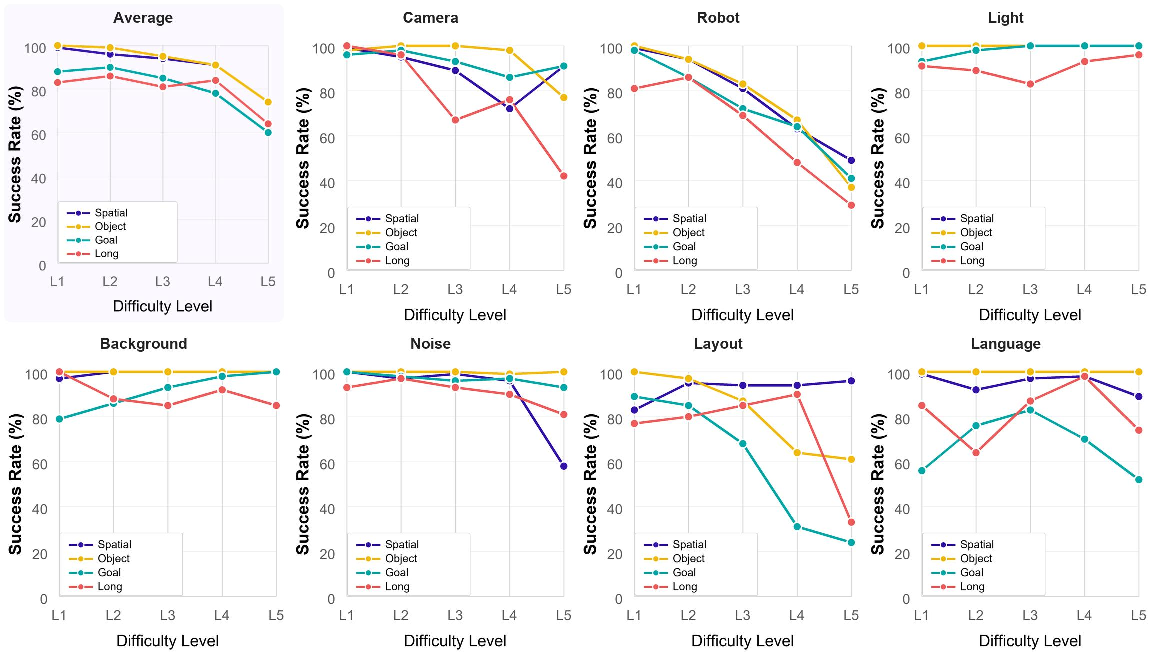
\includegraphics[width=\textwidth]{figures/suite_sr_contact_sheet.pdf}
    \caption{
    \textbf{Detailed zero-shot robustness on LIBERO-Plus.}
    We report success rates across difficulty levels L1--L5 for each perturbation category in the LIBERO-PLUS benchmark.
    The Average panel summarizes performance across all perturbation categories.
    }
    \label{fig:perturb_robustness}
\end{figure*}
\begin{table*}[t]
\centering
\caption{
\textbf{Per-task success rates on LIBERO Original.}
Task names are abbreviated by removing suite-level repeated context.
}
\label{tab:libero_original_per_task_sr_compact}
\small
\setlength{\tabcolsep}{4pt}
\renewcommand{\arraystretch}{1.02}
\resizebox{\textwidth}{!}{
\begin{tabular}{lc lc lc lc}
\toprule
\multicolumn{2}{c}{\textbf{Spatial} \; \textbf{98.6\%}} &
\multicolumn{2}{c}{\textbf{Object} \; \textbf{99.0\%}} &
\multicolumn{2}{c}{\textbf{Goal} \; \textbf{97.4\%}} &
\multicolumn{2}{c}{\textbf{Long} \; \textbf{94.6\%}} \\
\cmidrule(lr){1-2}\cmidrule(lr){3-4}\cmidrule(lr){5-6}\cmidrule(lr){7-8}
Task & SR & Task & SR & Task & SR & Task & SR \\
\midrule
Between plate \& ramekin & 100\% & Alphabet soup & 100\% & Open middle drawer & 100\% & Soup + tomato sauce to basket & 96\% \\
Next to ramekin & 100\% & Cream cheese & 98\% & Bowl on stove & 100\% & Cream cheese + butter to basket & 100\% \\
From table center & 98\% & Salad dressing & 100\% & Wine bottle on cabinet & 96\% & Stove on + moka pot on stove & 98\% \\
On cookie box & 100\% & BBQ sauce & 100\% & Top drawer open + bowl inside & 90\% & Bowl in bottom drawer + close & 100\% \\
In top drawer & 98\% & Ketchup & 98\% & Bowl on cabinet & 98\% & Mugs to left/right plates & 80\% \\
On ramekin & 96\% & Tomato sauce & 94\% & Plate to front of stove & 98\% & Book to caddy back compartment & 100\% \\
Next to cookie box & 100\% & Butter & 100\% & Cream cheese in bowl & 100\% & Mug to plate + pudding to plate & 96\% \\
On stove & 100\% & Milk & 100\% & Turn on stove & 100\% & Soup + cream cheese box to basket & 96\% \\
Next to plate & 94\% & Chocolate pudding & 100\% & Bowl on plate & 92\% & Both moka pots on stove & 88\% \\
On wooden cabinet & 100\% & Orange juice & 100\% & Wine bottle on rack & 100\% & Mug to microwave + close & 92\% \\
\bottomrule
\end{tabular}
}
\end{table*}


Table~\ref{tab:libero-plus-2x2} provides the suite-by-perturbation breakdown for LIBERO-Plus~\cite{fei2025libero}, expanding the aggregate LIBERO and LIBERO-Plus results reported in the main paper. Figure~\ref{fig:perturb_robustness} further breaks down LIBERO-Plus performance by perturbation difficulty level, showing how GAM behaves as each perturbation becomes more severe. Table~\ref{tab:libero_original_per_task_sr_compact} reports task-wise success rates on the original LIBERO~\cite{liu2023libero} benchmark.

Overall, these breakdowns show that GAM preserves strong performance on the original LIBERO tasks while improving robustness on LIBERO-Plus, especially under perturbations that require stable geometric understanding such as camera-viewpoint changes.

\subsection{Generated Future Depth Maps}
\label{sec:appendix-generated_depth}
\begin{figure*}[t]
    \centering
    \vspace{-0.35em}

    \begin{subfigure}[t]{0.95\textwidth}
        \centering
        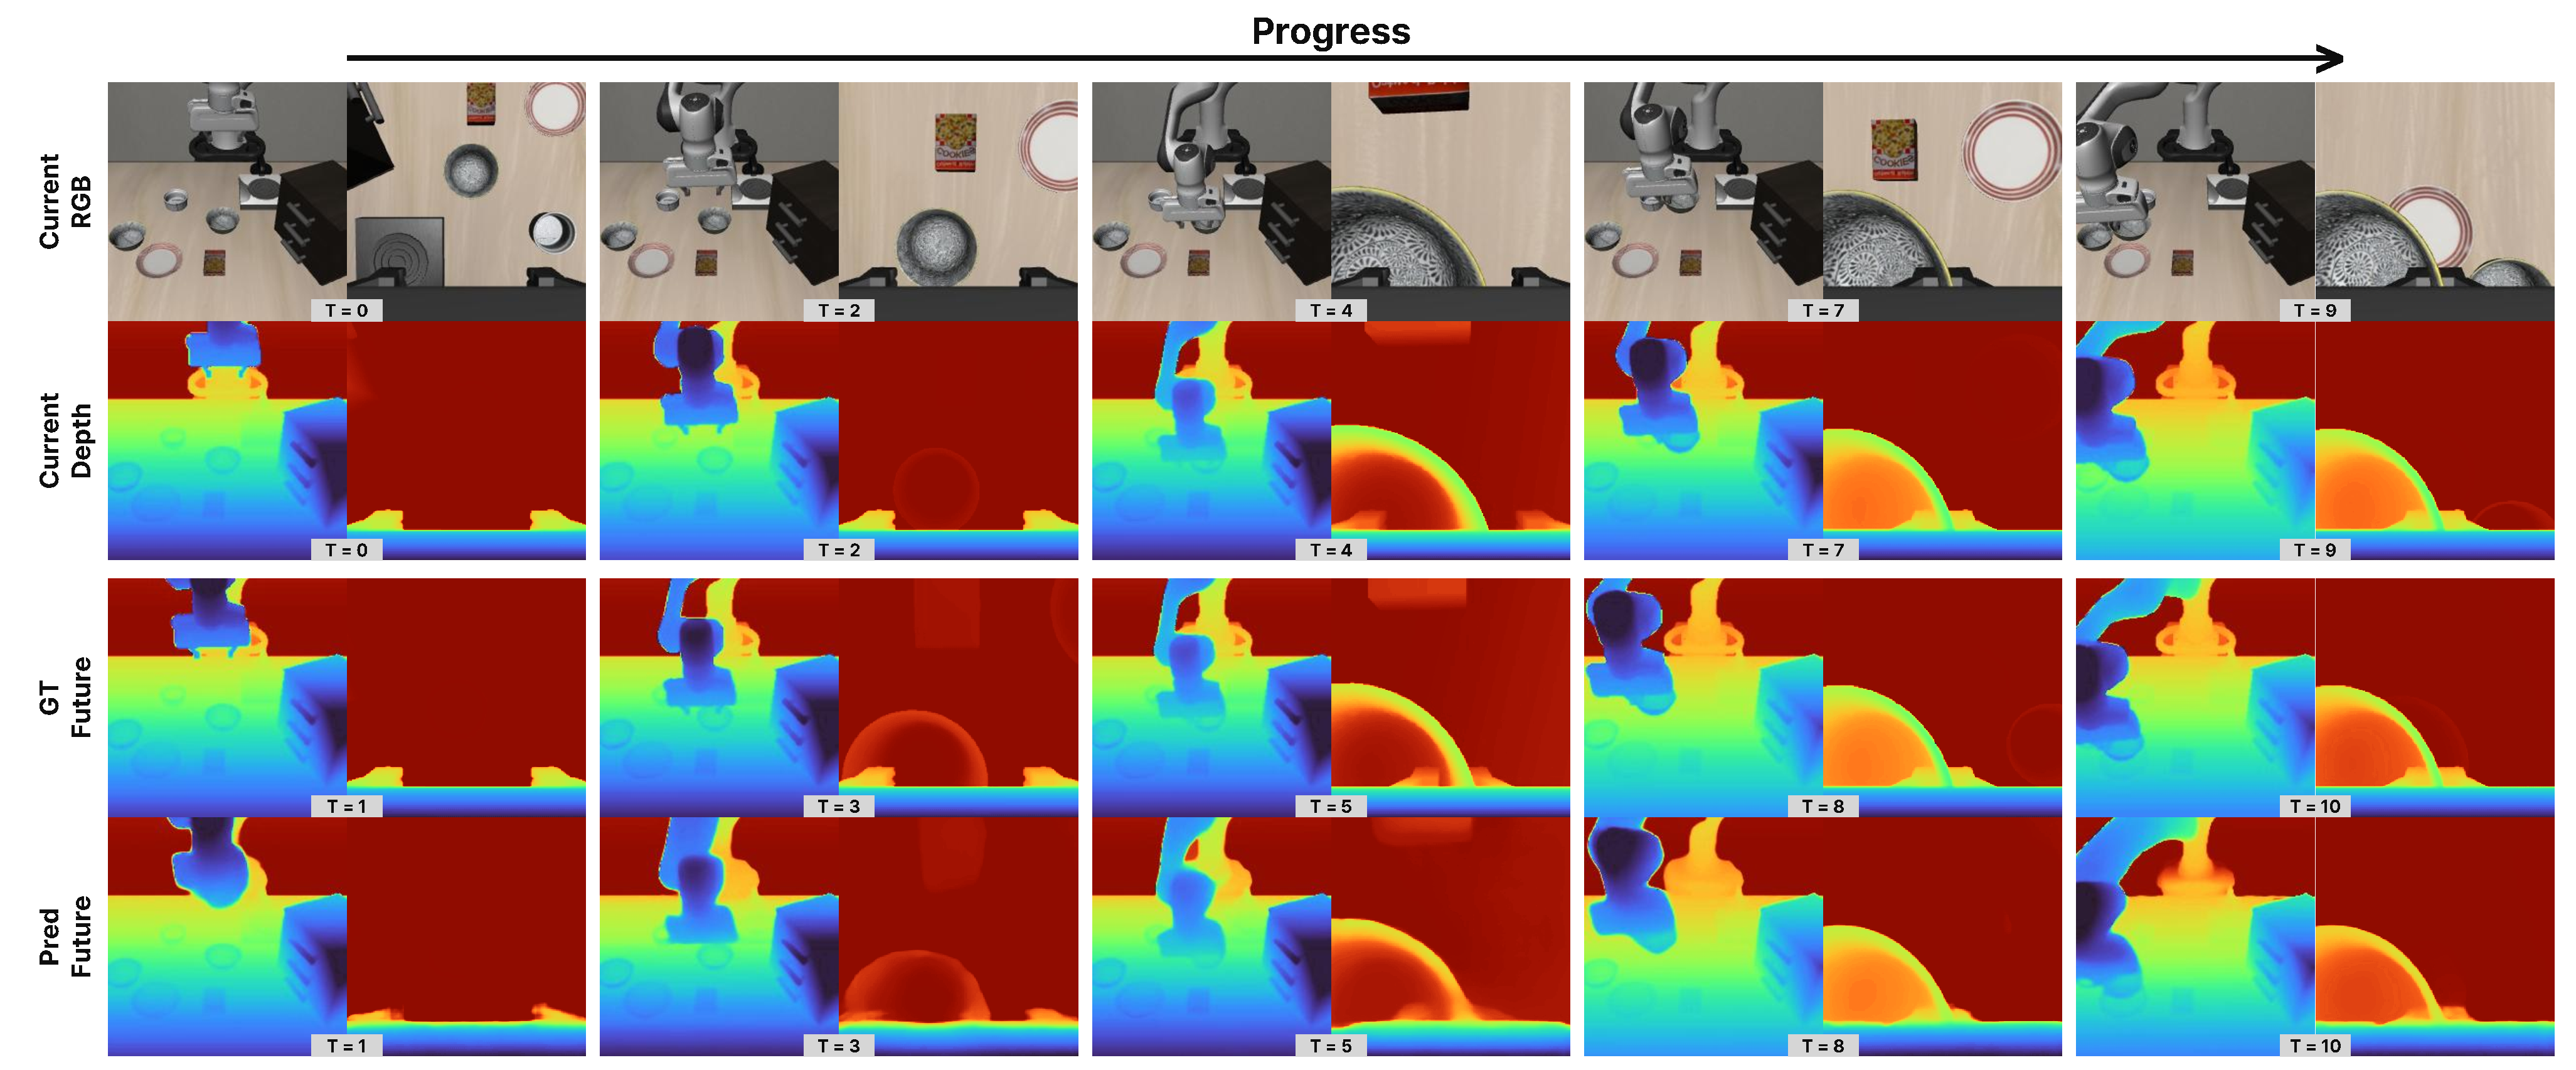
\includegraphics[width=0.95\linewidth]{figures/qual/libero_pair_layout_5step_editable-1.pdf}
        \caption{LIBERO-Spatial: bowl from table center to plate.}
        \label{fig:libero-spatial-depth-1}
    \end{subfigure}

    \vspace{-0.35em}

    \begin{subfigure}[t]{0.95\textwidth}
        \centering
        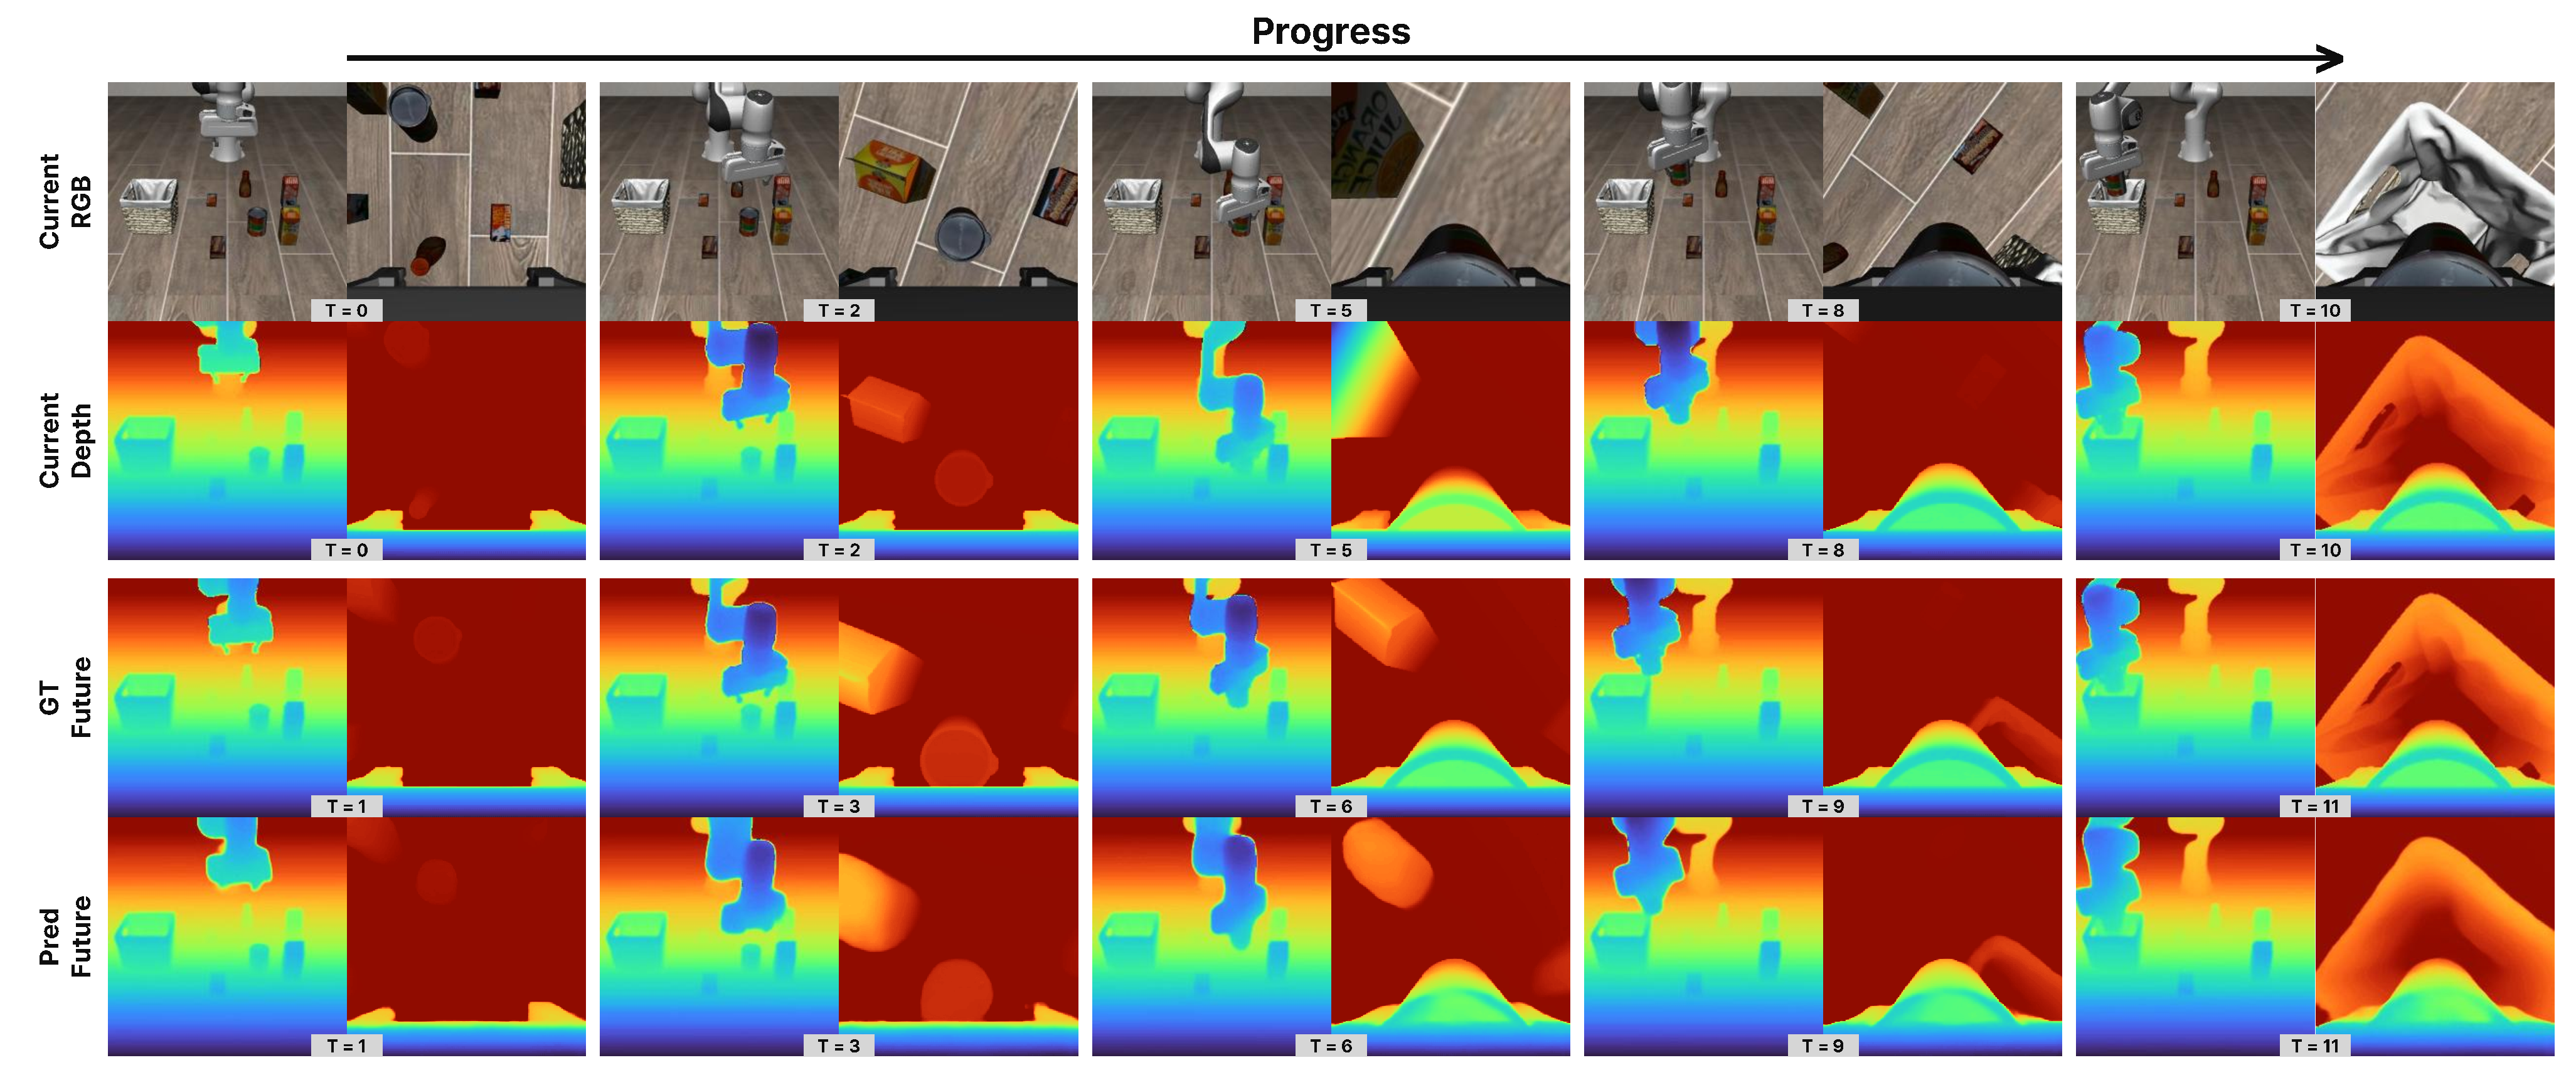
\includegraphics[width=0.95\linewidth]{figures/qual/libero_pair_layout_5step_editable-2.pdf}
        \caption{LIBERO-Object: tomato sauce to basket.}
        \label{fig:libero-object-depth-1}
    \end{subfigure}

    \vspace{-0.35em}

    \begin{subfigure}[t]{0.95\textwidth}
        \centering
        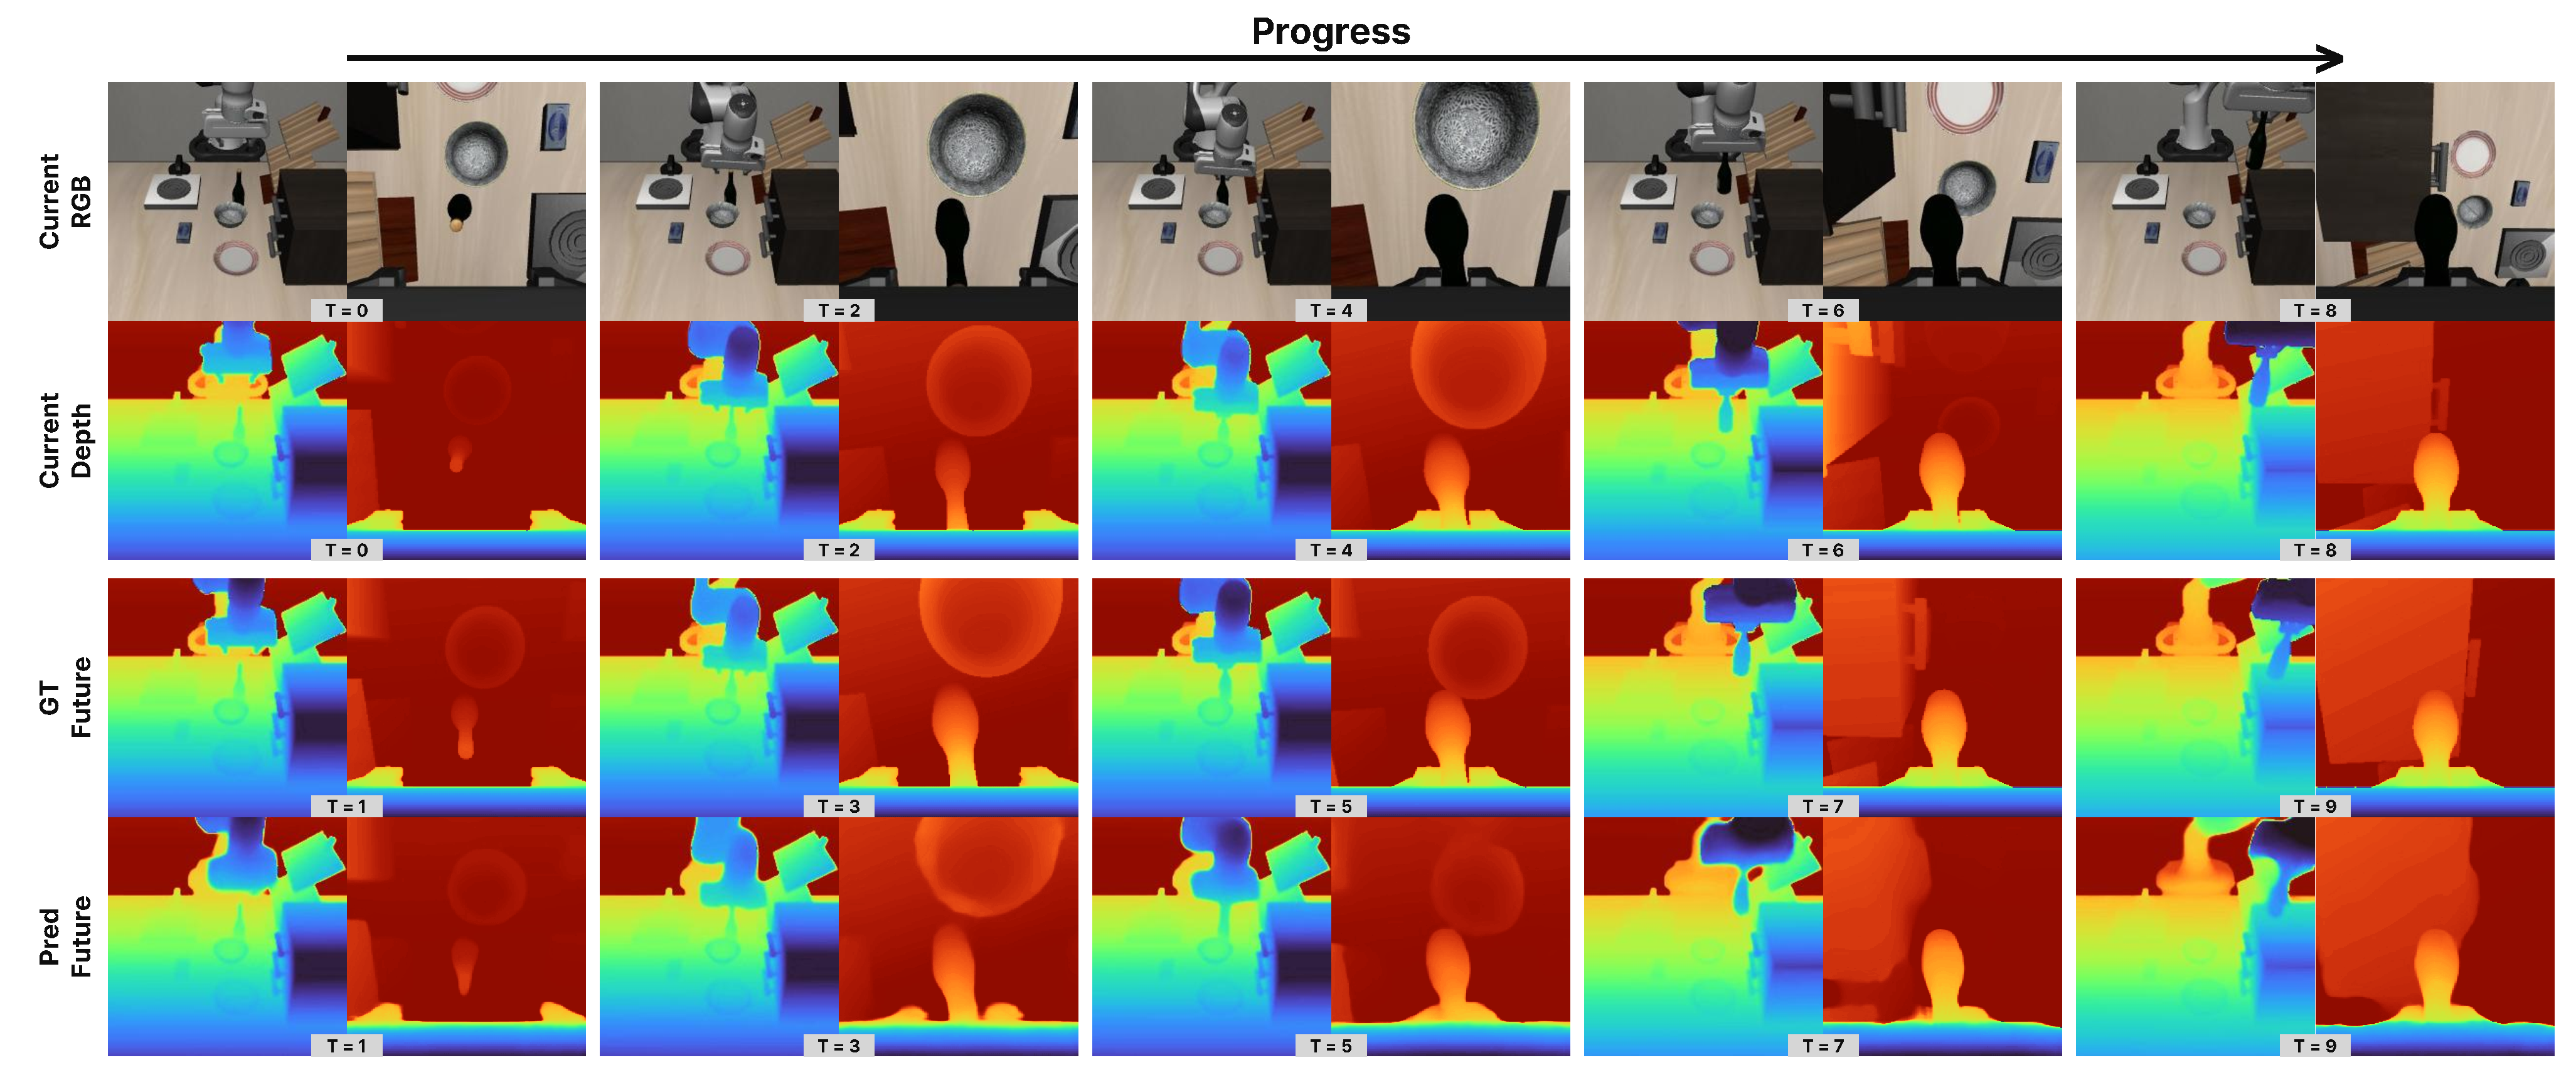
\includegraphics[width=0.95\linewidth]{figures/qual/libero_pair_layout_5step_editable-3.pdf}
        \caption{LIBERO-Long: cream cheese and butter to basket.}
        \label{fig:libero-long-depth-1}
    \end{subfigure}

    \vspace{-0.35em}

    \begin{subfigure}[t]{0.95\textwidth}
        \centering
        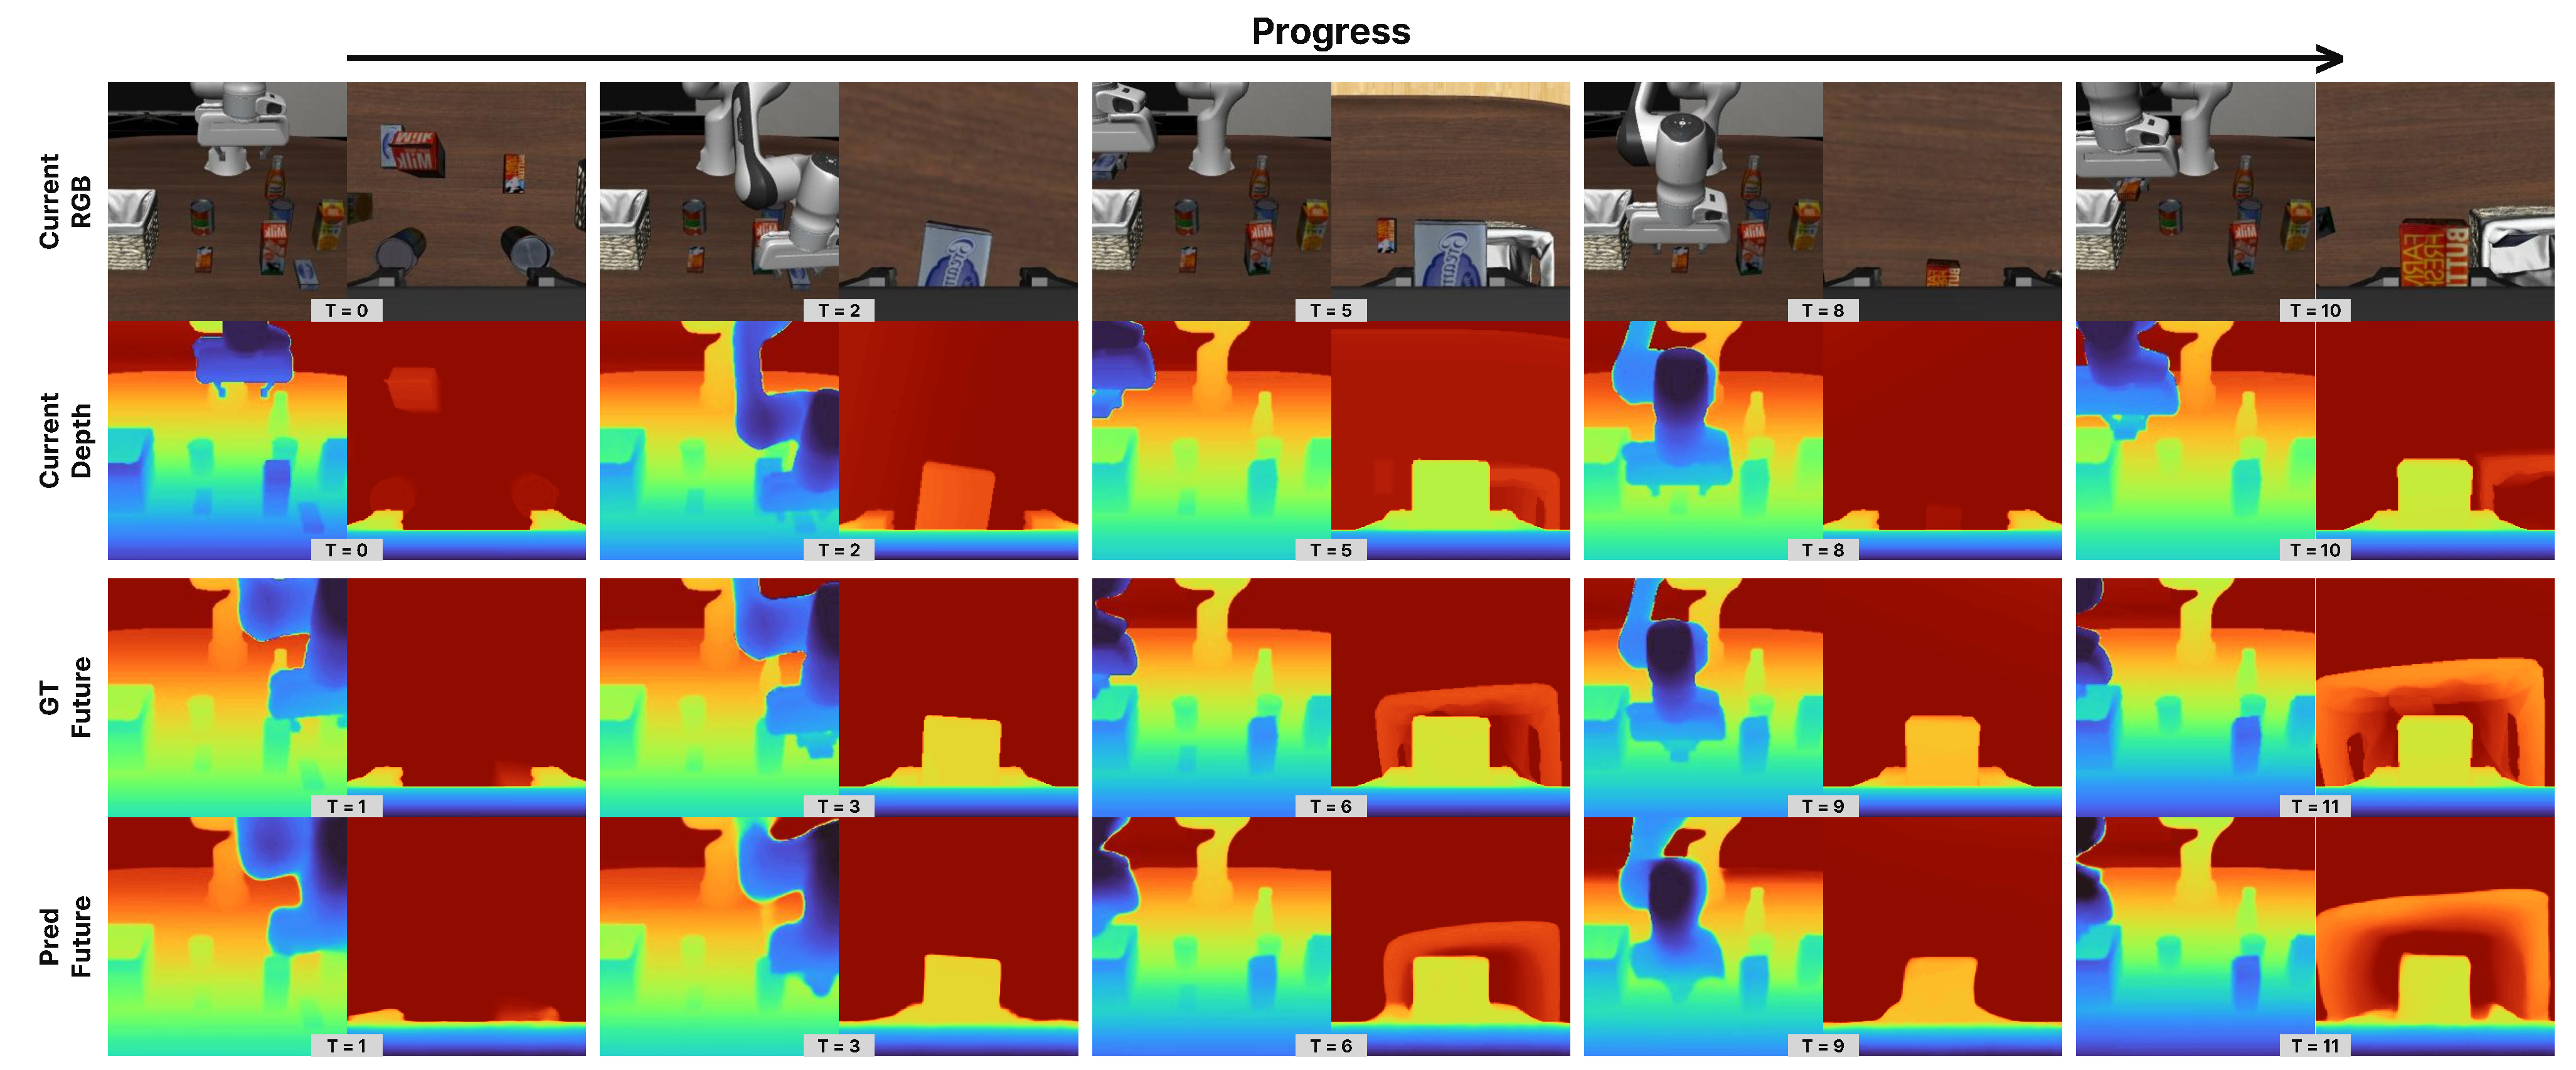
\includegraphics[width=0.95\linewidth]{figures/qual/libero_pair_layout_5step_editable-4.pdf}
        \caption{LIBERO-Goal: wine bottle on cabinet.}
        \label{fig:libero-goal-depth-1}
    \end{subfigure}
    \vspace{-5px}
    \caption{
    \textbf{Future depth visualizations predicted by our model on representative LIBERO tasks.}
    }
    \label{fig:libero_future_depth_visualizations}
\end{figure*}

In Figure~\ref{fig:libero_future_depth_visualizations}, we visualize the future depth predictions generated by GAM across each task suite in the LIBERO benchmark. Given a current RGB observation, GAM predicts the and future depth maps while simultaneously generating actions that align spatially with the anticipated future geometry. As demonstrated in the visualizations, GAM accurately forecasts the future depth alongside its corresponding action sequence.


\clearpage
\section{Ablation and Diagnostic Analyses}
\label{sec:appendix-ablation_analysis}


\subsection{When to Predict Actions?}
\label{sec:appendix-layer_ablation}


\begin{wraptable}{r}{0.43\textwidth}
    \vspace{-10pt}
    \centering
    \footnotesize
    \setlength{\tabcolsep}{3.5pt}
    \caption{\textbf{Direct action-token ablation.}}
    \label{tab:action_decoding_path_ablation}
    \begin{tabular}{lccc}
    \toprule
    Variant  & Orig. & Plus \\
    \midrule
    Direct-action supervision & 98.4 & 84.1 \\
    \textbf{GAM (Ours)}  & 99.6 & 89.7 \\
    \bottomrule
    \end{tabular}\vspace{-10pt}
\end{wraptable}

We additionally evaluate a direct-action supervision variant that applies the action loss directly to the output action token of the causal future predictor, without passing the action token through the remaining DA3 blocks. This ablation uses the same setting as the main component ablation on LIBERO-Object.
 
Passing the action token through the deep geometric decoder provides an additional improvement, particularly on LIBERO-Plus Object, suggesting that the remaining GFM layers contribute to refine the action representation, especially under camera perturbations.

\subsection{Attention Analysis}
\label{sec:appendix-attention_analysis}
In Figure~\ref{supfig:attention}, we visualize the attention maps of action tokens across GFM layers to inspect which visual regions contribute to action decoding. As shown in the attention maps, several intermediate layers attend to task-relevant regions, with clear saliency around manipulated objects and nearby contact regions. This qualitative trend is consistent with the layer ablation: mid-level representations retain object-level structure while still leaving enough depth in the GFM decoder for action-token refinement.

\begin{figure*}[t]
    \centering
    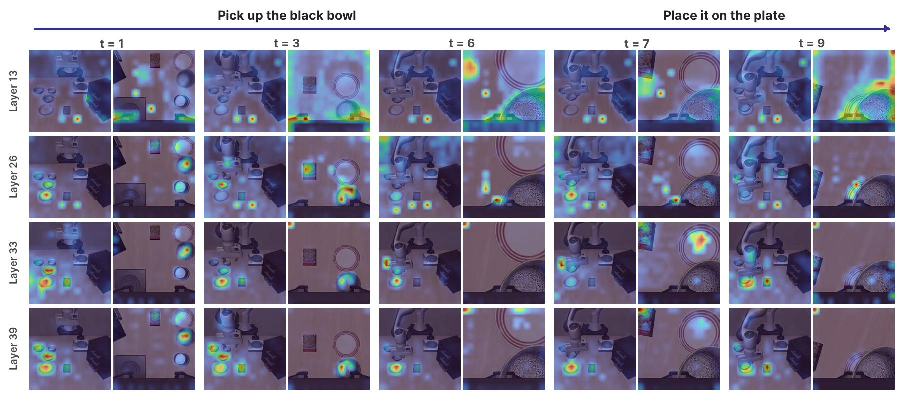
\includegraphics[width=\textwidth]{figures/attention_layers_timestep_subset_pretendard_v4.pdf}
    \caption{
    \textbf{Attention visualizations of action tokens.}
    }
    \label{supfig:attention}
\end{figure*}
